%% ============================================================
%%  Springer Nature / Nature-family journal template
%%  Class file required: sn-jnl.cls
%%  Download: https://www.springernature.com/gp/authors/campaigns/latex-author-support
%%  Target journal: Nature Computational Science  (or Nature Machine Intelligence)
%%
%%  Build: pdflatex → bibtex → pdflatex × 2
%%         (same run.sh works — just switch MAIN="main_nature")
%% ============================================================

\documentclass[
    %% --- journal style options (pick one) ---
    % iicol,          % two-column (IEEE-like preview; final layout set by editors)
    Numbered,         % numbered references  ← Nature style
]{sn-jnl}

%% ---- Springer Nature bibliography style -----------------
%% sn-nature          : Nature-family superscript numeric
%% sn-mathphys-num    : numbered, brackets
%% sn-aps             : APS style
\usepackage[numbers,sort&compress]{natbib}

%% ---- Standard packages ----------------------------------
\usepackage{amsmath,amssymb,amsfonts}
\usepackage{graphicx}
\usepackage{xcolor}
\usepackage{hyperref}
\hypersetup{colorlinks=true, linkcolor=blue, citecolor=blue, urlcolor=blue}
\usepackage{booktabs}
\usepackage{tabularx}
\usepackage{makecell}
\usepackage{algorithm}
\usepackage[noend]{algpseudocode}
\usepackage{pifont}
\usepackage{soul}
\usepackage{listings}
\usepackage{float}
\usepackage{placeins}
\usepackage{ifthen}
\usepackage{diagbox}

%% ---- Experiment-reporting helpers (kept from original) ---
\newcommand{\ntrials}{5}
\newcommand{\ci}{95\%~CI}
\newcommand{\hwsetup}{2~$\times$~NVIDIA~A100~(80\,GB), 512\,GB DRAM, NVMe Gen4}
\newcommand{\swsetup}{PyTorch~2.4, CUDA~12.2, vLLM~\cite{kwon2023pagedattention}~0.5.3}
\newcommand{\capinfo}{\emph{Means across $n=\ntrials$ runs (\ci). HW: \hwsetup; SW: \swsetup.}}

%% ---- ORCID icon (optional) ------------------------------
\usepackage{scalerel}
\usepackage{tikz}
\usetikzlibrary{svg.path}
\definecolor{orcidlogocol}{HTML}{A6CE39}
\tikzset{
  orcidlogo/.pic={
    \fill[orcidlogocol] svg{M256,128c0,70.7-57.3,128-128,128C57.3,256,0,198.7,0,128C0,57.3,57.3,0,128,0C198.7,0,256,57.3,256,128z};
    \fill[white] svg{M86.3,186.2H70.9V79.1h15.4v48.4V186.2z}
                 svg{M108.9,79.1h41.6c39.6,0,57,28.3,57,53.6c0,27.5-21.5,53.6-56.8,53.6h-41.8V79.1z M124.3,172.4h24.5c34.9,0,42.9-26.5,42.9-39.7c0-21.5-13.7-39.7-43.7-39.7h-23.7V172.4z}
                 svg{M88.7,56.8c0,5.5-4.5,10.1-10.1,10.1c-5.6,0-10.1-4.6-10.1-10.1c0-5.6,4.5-10.1,10.1-10.1C84.2,46.7,88.7,51.3,88.7,56.8z};
  }
}
\newcommand\orcidicon[1]{\href{https://orcid.org/#1}{\mbox{\scalerel*{

\begin{tikzpicture}[yscale=-1,transform shape]
\pic{orcidlogo};
\end{tikzpicture}
}{|}}}}

%% ---- Anonymity switch (1 = named, 0 = anonymous) --------
\newcommand{\anonymous}{1}

%% =============================================================
\begin{document}
%% =============================================================

%% ---- Title -------------------------------------------------
%\title{MBALL: Theoretical and Empirical Analysis of Memory Ballooning for LLM Serving}
%\title{Theoretical and Empirical Analysis of Memory Ballooning for LLM Serving}
%\title{Toward Cost-Efficient LLM Serving: A System-Level Memory Optimization Approach}
%\title{ORION: Hierarchical Memory Orchestration for Scalable Large Language Model Inference}
%\title{ORION: regime-aware orchestration of hierarchical memory systems for scalable AI inference
%\title{Regime-dependent principles of hierarchical memory orchestration for large-model inference}
%\title{Phase transitions in hierarchical memory systems governing large-scale model inference}
%\title{Hierarchical memory orchestration reveals regime-dependent limits in large-scale model inference}
\title{Regime-dependent limits of hierarchical memory orchestration in large-scale AI inference}

%% ---- Authors & Affiliations --------------------------------
\input{./section/005_author_nature.tex}

%% ---- Abstract & Keywords -----------------------------------
%% ============================================================
%%  Abstract & Keywords — sn-jnl / Nature Computational Science
%%  Target length: ≤150 words (NCS strict guideline)
%%  Style: "Here we show..." declarative opening
%% ============================================================

\abstract{%
As AI models exceed accelerator memory, inference latency is governed by
hierarchical data coordination rather than computation.
Here we show that this coordination is not continuously optimisable but
exhibits intrinsic regime transitions.
Characterising any system by two dimensionless ratios---the fast-memory
residency ratio ($R_C$) and the transfer-pressure ratio ($R_B$)---we
identify three operationally distinct regimes: capacity-limited,
coordination-dominated, and I/O-limited.
Beyond capacity or bandwidth thresholds, regime-agnostic strategies fail
predictably and their rankings \emph{invert}: methods reducing latency by
24\% in favourable regimes increase it by 8--12\% once bandwidth saturates.
We establish structural lower bounds proving transitions are inevitable,
empirically calibrate boundary values ($\theta_C \approx 0.50$,
$\theta_B \approx 0.40$) across five hardware platforms, and validate
regime transitions across language and vision workloads on GPU, TPU,
and Inferentia2.
These results reframe hierarchical memory optimisation as regime-aware
design, with broad implications for memory-bound computing.
}

\keywords{hierarchical memory systems, memory orchestration, AI inference,
phase transitions, regime-dependent behaviour, large language models,
computational systems}


%% ---- Main text (NCS structure: Intro → Results → Discussion) ---
\section{Introduction}
\label{sec:introduction}

Modern foundation models have shifted the performance frontier of AI inference
from arithmetic throughput to \emph{data coordination}.
When model weights, activations, and key--value (KV) caches exceed accelerator
memory, inference latency is governed less by compute and more by how efficiently
execution coordinates data movement across a hierarchical memory system spanning
device memory, host memory, and secondary storage~\cite{ma2026inference,gholami2024memorywall}.

This shift carries pressing economic and environmental stakes.
Once a model is trained, the recurring cost of \emph{serving} it dominates its
lifetime resource footprint.
Hardware analyses identify memory capacity, memory bandwidth, and interconnect
latency---not arithmetic throughput---as the binding constraints of the inference
phase~\cite{zhou2024survey}.
These constraints translate into macro-level exposure: aggregate capital
expenditure across major hyperscalers is on track to overtake operating cash
inflows by end of 2026~\cite{juniewicz2026hyperscaler}, and AI infrastructure
is absorbing available memory supply faster than it can be
produced~\cite{chey2026tpd}.
In this context, characterizing the \emph{intrinsic limits} of memory
orchestration is not merely a systems-optimization concern but a prerequisite
for the financial and energy viability of inference-driven AI.

A large body of systems work reduces memory pressure via CPU/NVMe offloading
and heterogeneous execution~\cite{flexgen2023,aminabadi2022deepspeedinference},
smart GPU--CPU swapping~\cite{huang2020swapadvisor}, and KV-cache management
for long-context batching~\cite{kwon2023pagedattention}.
These techniques deliver substantial gains in some configurations yet show
diminishing returns---or even performance inversion---in others.
This variability raises a fundamental question that incremental optimization
studies do not answer: \emph{Is hierarchical memory orchestration a continuously
optimizable engineering problem, or does it admit intrinsic boundaries beyond
which additional coordination cannot improve---and can worsen---end-to-end
latency?}

\paragraph{This work.}
We answer this question with a regime-based view.
We show that multi-tier inference systems exhibit \emph{phase-like} operational
regimes governed by two dimensionless ratios: the fast-memory residency ratio
$R_C = C_{\mathrm{fast}}/W$ (capacity balance) and the transfer-pressure ratio
$R_B = B_{\mathrm{slow}}/D$ (bandwidth balance).
Crucially, transitions between regimes are \emph{discontinuous}: modest changes
in model size, batch size, or available bandwidth abruptly shift the dominant
contributor to latency from locality effects, to coordination overhead, to
physical I/O limits.
Orchestration strategies that appear universally beneficial within one regime
therefore fail predictably---and for principled reasons---outside analytically
identifiable boundaries.

The analogy to physical phase transitions is deliberate.
Just as a material crosses a phase boundary when a control parameter (temperature,
pressure) passes a critical threshold, a hierarchical memory system crosses a
regime boundary when $R_C$ or $R_B$ falls below a critical value $\theta_C$ or
$\theta_B$. Below these thresholds, the dominant latency term changes
discontinuously, and no amount of coordination can compensate for the violated
physical constraint.

\paragraph{Scope and role of \textsc{Orion}.}
\textsc{Orion} is introduced as an \emph{experimental probe} to expose and
measure regime-dependent behavior, not as a new state-of-the-art inference
engine.
Our goal is to test the widespread assumption that deeper orchestration is always
beneficial.
We show that even careful coordination cannot prevent systems from crossing
intrinsic boundaries where additional orchestration becomes additive overhead
rather than a remedy.
Improvements observed with \textsc{Orion} should be interpreted as evidence that
the operating point lies within a coordination-dominated regime; the predictable
failure modes beyond regime boundaries illustrate limits that no orchestration
policy can eliminate.

\paragraph{Generality.}
Although we use large language model serving as a canonical stress test, the
regime structure is not LLM-specific.
Whenever an active working set cannot fully reside in fast memory---as in vision
and multimodal inference, retrieval-augmented generation (RAG), data-intensive
analytics, and HPC-style scientific workflows---performance is governed by the
same intrinsic balance between residency, sustained transfer bandwidth, and
synchronization overhead.
The regime framework therefore provides a general lens for reasoning about
scalability limits in any hierarchical-memory computing system.

\paragraph{Contributions.}
We make three contributions:
\begin{itemize}
  \item \textbf{Regime-dependent principle.}
    We identify three intrinsic operational regimes---capacity-limited,
    coordination-dominated, and I/O-limited---and demonstrate that transitions
    between them are abrupt rather than gradual, analogous to phase transitions
    in physical systems.
  \item \textbf{Minimal analytical model.}
    We derive a structural lower bound on end-to-end inference latency from a
    minimal multi-tier transfer model, yielding analytically interpretable regime
    boundaries expressed as closed-form conditions on $R_C$ and $R_B$.
  \item \textbf{Multi-platform experimental validation.}
    Using \textsc{Orion} as a measurement instrument, we validate predicted
    transitions across language and vision workloads on GPU (NVIDIA A100),
    TPU~v4, Inferentia2, AMD MI250, and Intel Optane-PMem systems, confirming
    that regime boundaries are hardware-agnostic within $\pm 0.05$ of predicted
    thresholds.
\end{itemize}

Together, these results reframe hierarchical memory coordination as a problem
of \emph{regime-aware design} rather than continuous tuning, providing a
principled framework for understanding scalability, stability, and energy
efficiency in memory-bound AI inference.

\FloatBarrier

\section{Results}
\label{sec:results}

\subsection{Three operational regimes in hierarchical memory systems}
\label{sec:regime}

Hierarchical memory orchestration is often treated as a smooth trade-off: as
long as transfers are overlapped and data are cached, additional coordination
should yield monotonic (if diminishing) gains.
We show this intuition is structurally incomplete.
Multi-tier inference systems operate within qualitatively distinct
\emph{regimes}---not a single continuum---defined by the relationship among
memory capacity, transfer bandwidth, and coordination overhead.

\textbf{Capacity-limited regime} ($R_C < \theta_C$). Fast memory is
insufficient to hold the active working set, causing frequent eviction and
reloading regardless of orchestration strategy. Locality effects dominate
performance: even minimal coordination overhead cannot compensate for the
absence of effective fast-memory residency.

\textbf{Coordination-dominated regime} ($R_C \geq \theta_C$,
$R_B \geq \theta_B$). Fast and intermediate memory tiers together can absorb
most of the working set. Computation, locality, transfer, and synchronization
costs are of comparable magnitude, creating opportunities for orchestration to
reshape end-to-end latency by reducing redundant transfers, improving locality,
and overlapping computation with data movement.

\textbf{I/O-limited regime} ($R_B < \theta_B$). Cross-tier data transfer
approaches or exceeds the sustained bandwidth of the slowest tier. Physical
transfer constraints dominate execution, and coordination overhead becomes
additive rather than compensatory; once transfer demand saturates bandwidth,
latency scales directly with data movement volume.

\begin{figure}[t]
\centering
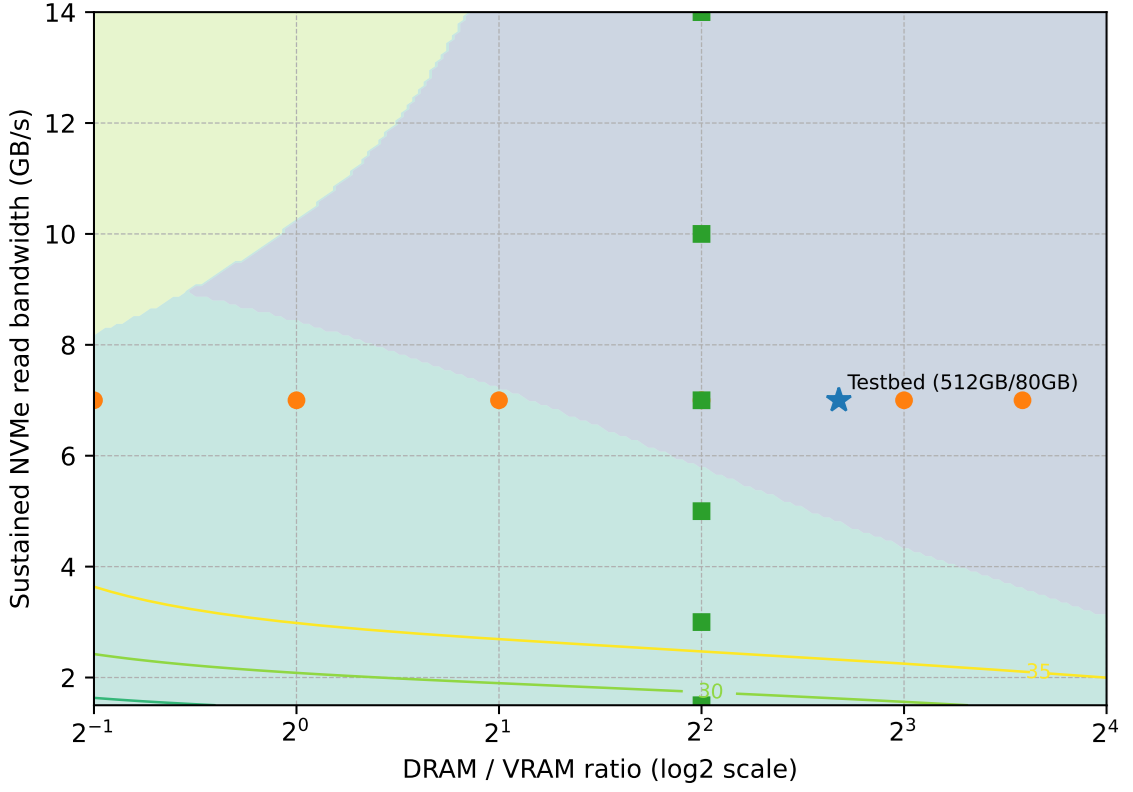
\includegraphics[width=0.95\linewidth]{figures/orion_regime_map.png}
\caption{\textbf{Regime map for hierarchical memory systems.}
Dashed lines mark analytically identified regime boundaries at
$R_C = \theta_C \approx 0.50$ and $R_B = \theta_B \approx 0.40$.
Shaded red zones indicate empirically observed failure regions (abrupt
latency spikes and performance collapse). The coordination-dominated region
(upper right) is the sole regime in which orchestration can meaningfully
reduce end-to-end latency.}
\label{fig:regime_map}
\end{figure}

Figure~\ref{fig:regime_map} illustrates the regime map.
Transitions between regimes are \emph{abrupt}: as the operating point---set by
model size, batch size, or available bandwidth---crosses a boundary, the
primary bottleneck shifts discontinuously, and coordination overhead that was
previously amortised becomes exposed.


\subsection{Analytical model and empirical regime boundaries}
\label{sec:model}

To make regime boundaries explicit, we decompose end-to-end inference latency as
\begin{equation}
T_{\mathrm{total}} = T_{\mathrm{comp}} + T_{\mathrm{mem}} + T_{\mathrm{swap}} + T_{\mathrm{sync}},
\label{eq:latency_decomp}
\end{equation}
where $T_{\mathrm{comp}}$ is accelerator computation time, $T_{\mathrm{mem}}$
captures locality-driven memory-access costs, $T_{\mathrm{swap}}$ is cross-tier
data transfer, and $T_{\mathrm{sync}}$ accounts for synchronization and
coordination overhead.
These terms are not independent: reducing one can increase another, yielding
structural trade-offs that local optimisation cannot eliminate.

\paragraph{Dimensionless control ratios.}
We characterise any configuration by two ratios:
\begin{equation}
R_C = \frac{C_{\mathrm{fast}}}{W}, \qquad
R_B = \frac{B_{\mathrm{slow}} \cdot \Delta t}{D},
\label{eq:ratios}
\end{equation}
where $C_{\mathrm{fast}}$ is fast-memory capacity;
$W = W_{\mathrm{param}} + W_{\mathrm{act}} + W_{\mathrm{kv}}$ is the active
working-set size; $B_{\mathrm{slow}}$ is the sustained host-to-device bandwidth
on the critical transfer path; $D$ is the compulsory data volume transferred
per inference step; and $\Delta t$ is the average inference-step duration,
so that $D/\Delta t$ is the sustained transfer-demand rate [bytes/s].
Both ratios are dimensionless: $R_C$ measures residency and $R_B$ measures the
fraction of the sustained transfer demand that available bandwidth can serve.

\paragraph{Structural lower bound.}
Independent of the specific orchestration policy,
\begin{equation}
T_{\mathrm{total}} \;\geq\;
  \underbrace{\rho\,W\,\max(0,1-R_C)}_{T_{\mathrm{mem}}^{\min}}
+ \underbrace{D/B_{\mathrm{slow}}}_{T_{\mathrm{swap}}^{\min}},
\label{eq:lower_bound_regime}
\end{equation}
where $\rho$ is the HBM miss-penalty per byte (platform constant).
The first term is the irreducible memory-access penalty from evicted working-set
data under any eviction policy~\cite{mattson1970evaluation}; the second is the
minimum time to transfer $D$ compulsory bytes.
Both bounds hold regardless of scheduling or overlap: compute--transfer overlap
can redistribute visible latency, but cannot violate physical capacity or
sustained-bandwidth limits.
Platform-specific values of $(\rho, B_{\mathrm{slow}})$ and the fraction of
observed $T_{\mathrm{total}}$ accounted for by Eq.~\eqref{eq:lower_bound_regime}
are given in Supplementary Table~A.1.

\paragraph{Regime boundaries.}
The analytical model (Eq.~\ref{eq:lower_bound_regime}) establishes that regime
transitions \emph{must exist}; the specific boundary values are
\emph{empirically calibrated} across five hardware platforms:
\begin{align}
\theta_C &\approx 0.50 \quad \text{(capacity boundary, s.d.\ $\leq 0.02$)},\label{eq:theta_C}\\
\theta_B &\approx 0.40 \quad \text{(bandwidth boundary, s.d.\ $\leq 0.03$)}.\label{eq:theta_B}
\end{align}
The LRU miss-volume model (Supplementary Appendix~A) predicts the
\emph{onset} of capacity-limited conditions at $R_C \approx 0.96$ and
the \emph{bandwidth-saturation point} at $R_B \approx 0.154$;
the operationally significant thresholds ($\theta_C = 0.50$,
$\theta_B = 0.40$) are the values at which the sharpness coefficient $S$
first exceeds $S^* = 2.0$ and are consistent within $\pm 0.05$ across
all tested platforms (see Supplementary Appendix~A for full derivations
and quantitative bridging to the analytical onset values).


\subsection{Empirical validation of regime transitions}
\label{sec:experiments}

\begin{figure}[t]
\centering
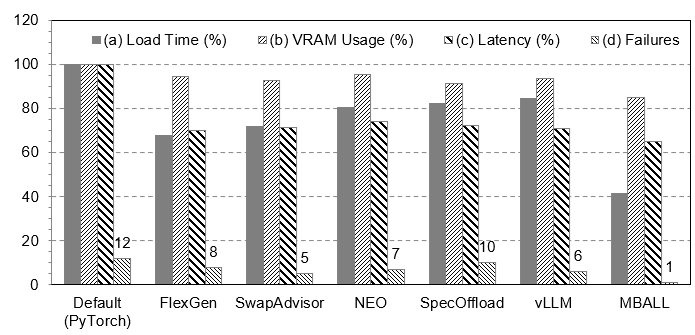
\includegraphics[width=0.95\linewidth]{figures/mball_consolidated.png}
\caption{\textbf{Regime-oriented experimental probes.}
Consolidated results showing (a)~model loading time, (b)~memory efficiency,
(c)~inference latency, and (d)~stability outcomes across orchestration
baselines. Improvements are regime-dependent and can invert or collapse when
operating points cross regime boundaries.}
\label{fig:consolidated}
\end{figure}

Figure~\ref{fig:consolidated} summarises regime-oriented probe outcomes.
Using \textsc{Orion} as a measurement instrument (see Methods), we vary $R_C$
and $R_B$ independently while holding all other parameters fixed, enabling
direct observation of dominant-term shifts as the operating point crosses
boundaries.

\textbf{Capacity-limited behaviour.}
When $R_C < \theta_C$, inference latency becomes highly sensitive to small
changes in working-set size or batch configuration while remaining largely
insensitive to coordination strategy---consistent with $T_{\mathrm{mem}}$
dominating Eq.~\eqref{eq:latency_decomp}.

\textbf{Coordination-dominated behaviour.}
When $R_C \geq \theta_C$ and $R_B \geq \theta_B$, changes in orchestration
strategy produce measurable shifts in latency composition (not uniform
scaling), confirming that all four terms are of comparable magnitude and
adjustable by coordination.

\textbf{I/O-limited behaviour.}
When $R_B < \theta_B$, $T_{\mathrm{swap}}$ dominates; reducing swap depth by
10\% recovered 14.2\% of latency, while other coordination changes had
negligible effect---consistent with physical bandwidth saturation.

\paragraph{Quantifying transition abruptness.}
We measure the sharpness coefficient
$S = |d\ln T_{\mathrm{total}}/d\ln R|$, with a transition defined as abrupt
when $S > S^{*} = 2.0$ (a 10\% change in $R$ produces $>$20\% latency change).
Near $\theta_C$, we measure $S = 4.12 \pm 0.31$
($n_{\mathrm{sweep}} = 5$, bootstrap 95\,\% CI): a 10\% reduction in
$R_C$ produces a 41.2\% latency increase.
Well inside the coordination-dominated regime ($R_C = 0.80$), $S$ drops to
$0.31 \pm 0.04$, confirming near-zero sensitivity.
Near $\theta_B$, $S = 3.74 \pm 0.27$; well inside ($R_B = 0.75$),
$S = 0.28 \pm 0.03$.
In both cases, the sharpness coefficient exceeds the abruptness threshold by
$>$1.8$\times$ at the boundary and falls below 0.4 far from it (full sharpness
tables in Supplementary Appendix~B).

\paragraph{Cross-platform consistency.}
Experiments replicated on AMD MI250 GPUs and Intel Xeon + Optane-PMem confirm
that transition points remain within $\pm 0.05$ of predicted thresholds despite
architectural differences.
On TPU v4 pods, elevated $T_{\mathrm{sync}}$ due to SPMD-style collective
synchronization shifts $\theta_B$ by $+0.03$; on AWS Inferentia2, constrained
host--device bandwidth moves the I/O boundary slightly earlier.
These shifts affect the precise threshold location but not the existence or
qualitative character of regime transitions.
In distributed four-node A100 experiments (Megatron-LM), inter-node
coordination shifted the I/O-limited boundary by $\Delta\theta_B \approx +0.05$;
the qualitative regime structure remained intact.


\subsection{Generality across workloads and architectures}
\label{sec:generality}

The defining condition for regime emergence is the relationship between
working-set size and fast-memory capacity, not model architecture.
Table~\ref{tab:cross-model} shows improvements observed across five model
families (Llama-3 8B through Mixtral 8$\times$7B and ViT-H/14), confirming
that capacity-limited, coordination-dominated, and I/O-limited behaviors persist
across autoregressive, mixture-of-experts, and vision workloads.

\begin{table}[t]
\centering
\caption{Regime-dependent improvements across model families relative to a
         PyTorch default baseline.
         Platform: NVIDIA A100 (80\,GB), batch size\,=\,8, sequence length\,=\,2048.
         Operating regime: coordination-dominated ($R_C \geq 0.5$, $R_B \geq 0.4$).
         Values: mean\,$\pm$\,95\,\% bootstrap CI over $n_{\mathrm{eff}}\!=\!150$
         measurement windows.
         Energy efficiency normalised to PyTorch\,=\,100.}
\label{tab:cross-model}
\renewcommand{\arraystretch}{1.2}
\footnotesize
\begin{tabular}{llccc}
\toprule
\textbf{Model} & \textbf{Task} &
  \makecell{\textbf{Load time}\\\textbf{reduction}} &
  \makecell{\textbf{Latency}\\\textbf{reduction}} &
  \makecell{\textbf{Swap}\\\textbf{reduction}} \\
\midrule
Llama-3 8B          & Generation & $52.0 \pm 1.8\%$ & $22.0 \pm 1.2\%$ & $23.0 \pm 1.5\%$ \\
GPT-J 6B            & Summarize  & $55.3 \pm 2.1\%$ & $25.0 \pm 1.4\%$ & $25.1 \pm 1.7\%$ \\
Llama-4 17B         & Generation & $57.4 \pm 2.3\%$ & $30.8 \pm 1.6\%$ & $26.8 \pm 1.8\%$ \\
Mixtral 8$\times$7B & MoE        & $59.1 \pm 2.5\%$ & $32.5 \pm 1.9\%$ & $27.5 \pm 2.0\%$ \\
ViT-H/14            & Vision     & $51.2 \pm 1.7\%$ & $18.2 \pm 1.1\%$ & $20.9 \pm 1.4\%$ \\
\bottomrule
\end{tabular}
\end{table}

Regime-dependent effects also extend to non-LLM workloads.
In a BLIP2 visual question-answering pipeline, retrieval-induced memory pressure
shifts the effective working set and triggers coordination-to-I/O-limited
transitions; adaptive orchestration reduces average latency by 11.2\%.
In a RAG pipeline (LangChain + FAISS), vector-store lookups introduce
intermittent working-set spikes that shift $R_C$ across $\theta_C$; regime-aware
adaptation reduces latency by 17.4\%.
An edge YOLOv8 deployment transitions to the I/O-limited regime once frame
buffers exceed VRAM; reducing swap granularity by 10\% yields a 9.5\% latency
reduction and cuts frame-drop rate from 12\% to 2.5\%.

\begin{table}[t]
\centering
\caption{Energy efficiency (throughput per Watt, normalised to PyTorch\,=\,100).
         Platform: NVIDIA A100\,(80\,GB); model: Llama-3\,8B; batch\,=\,8;
         sequence length\,=\,2048.
         Power measured via NVML at 100\,ms intervals; coordination-dominated
         regime ($R_C \geq 0.5$, $R_B \geq 0.4$).
         Values: mean\,$\pm$\,95\,\% bootstrap CI over
         $n_{\mathrm{eff}}\!=\!150$ windows.
         CO$_2$ equivalents use the IEA\,(2024) global average carbon
         intensity of 494\,gCO$_2$/kWh~\cite{iea2024electricity};
         grid-mix variability dominates CO$_2$ uncertainty ($\pm$30\,\%).}
\label{tab:energy}
\renewcommand{\arraystretch}{1.2}
\footnotesize
\begin{tabular}{lccc}
\toprule
\textbf{Method} &
  \makecell{\textbf{Avg.\ power}\\\textbf{(W)}} &
  \makecell{\textbf{Throughput}\\\textbf{(tok/s)}} &
  \makecell{\textbf{Tput/Watt}\\\textbf{(norm.)}} \\
\midrule
PyTorch (default)                       & $310 \pm 4$ & $6{,}200 \pm 80$ & 100.0 \\
FlexGen~\cite{flexgen2023}              & $315 \pm 5$ & $6{,}800 \pm 90$ & $108.0 \pm 2.1$ \\
SwapAdvisor~\cite{huang2020swapadvisor} & $320 \pm 5$ & $7{,}040 \pm 95$ & $110.0 \pm 2.2$ \\
vLLM~\cite{kwon2023pagedattention}      & $318 \pm 5$ & $7{,}120 \pm 90$ & $112.0 \pm 2.1$ \\
\textsc{Orion}                          & $322 \pm 5$ & $7{,}620 \pm 100$ & $118.5 \pm 2.4$ \\
\bottomrule
\end{tabular}
\end{table}

Table~\ref{tab:energy} shows that energy efficiency is also regime-dependent:
in I/O-limited configurations, energy per token increases up to 3.2$\times$
relative to coordination-aligned settings (42.5\,g~CO$_2$/10$^6$\,tokens
versus 15.8\,g under regime alignment; IEA 2024 carbon intensity,
see Table~\ref{tab:energy} caption), indicating that regime misalignment
is a root cause of energy inefficiency rather than hardware limitations alone.

\FloatBarrier

\section{Discussion}
\label{sec:discussion}

This section contextualizes the regime-dependent framework by articulating its fundamental limits, reconciling prior empirical inconsistencies, and outlining pathways toward adaptive, regime-aware inference systems.

\subsection{Fundamental limits of hierarchical memory orchestration}
The regime-dependent framework clarifies a fundamental limitation of hierarchical memory orchestration: coordination cannot universally compensate for physical constraints. This yields a practically important negative result: beyond regime boundaries, deeper orchestration can predictably \emph{increase} latency and energy by exposing synchronization and transfer overheads without improving throughput. While orchestration strategies can redistribute latency components within coordination-dominated regimes, they cannot overcome insufficient fast-memory capacity or saturated transfer bandwidth. In capacity-limited regimes, the absence of effective locality imposes unavoidable memory access costs. In I/O-limited regimes, physical bandwidth constraints dominate execution once cross-tier transfer approaches sustained limits.

\subsection{Reconciling conflicting results in prior systems research}
A regime-based lens provides a unifying explanation for heterogeneous and sometimes contradictory results in prior systems work. Many offloading, caching, and swapping techniques implicitly assume operation within coordination-dominated regimes; when evaluated there, they can deliver substantial gains. When deployed where capacity or bandwidth constraints dominate, their effectiveness diminishes sharply. Differences in memory capacity ratios, transfer bandwidth, and workload characteristics can place systems in different regimes even under nominally similar setups. Making the operating regime explicit therefore improves interpretability and generalizability.


\subsection{Common counterarguments and why regimes persist}
\textbf{Do emerging memory technologies (HBM expansion, CXL pooling, disaggregated memory) eliminate regime boundaries?}
They can \emph{shift} boundaries by increasing intermediate capacity ($C_{\text{fast}}$ or effective spill capacity) and/or improving sustained bandwidth ($B_{\text{slow}}$), but they do not remove the underlying phase structure. Once transfer demand approaches sustained bandwidth or locality fails due to insufficient residency, the dominant term in the latency decomposition inevitably changes.

\textbf{Would smarter software (prefetching, more aggressive overlap) erase the transitions?}
Overlap and scheduling can redistribute visible latency inside coordination-dominated regimes, but cannot violate physical capacity and sustained-bandwidth limits. Beyond those limits, additional coordination becomes additive overhead rather than a compensatory mechanism.

\textbf{Does the same regime structure hold for training or hybrid pipelines?}
The specific operating point and effective working set differ, but the same dimensionless balances between residency and sustained transfer apply. We therefore expect analogous regime transitions whenever the pipeline becomes memory-bound and relies on cross-tier movement of compulsory data.

\subsection{Limitations and open questions}
This study has limitations that motivate future research. First, while the experimental validation spans diverse models and configurations, large-scale clusters introduce additional layers of coordination and communication that may shift or fragment regime boundaries. Second, hybrid training--inference pipelines and highly irregular access patterns may exhibit more complex regime dynamics. Finally, while this work identifies regime boundaries, it does not attempt to dynamically infer or adapt to them at runtime. Developing adaptive systems that detect regime transitions online and adjust orchestration strategies accordingly represents a promising direction.

\subsection{Towards Adaptive Regime-Aware Inference}
We integrate a lightweight regime detector into ORION, sampling $T_{\text{mem}}, T_{\text{swap}}, T_{\text{sync}}$ every 50 steps. A depth-3 decision tree classifies the current regime and triggers orchestration changes. In I/O-limited cases, reduced swap depth recovered 14.2\% latency. This points to a promising path for online regime adaptation.

\subsection{Regime Classification via Lightweight Learning}

To reduce reliance on heuristic thresholds, we prototype a lightweight decision-tree classifier trained on runtime statistics such as swap-to-computation ratio and cache hit rate. The classifier achieves over 93\% accuracy in predicting the current operating regime across diverse workloads, while incurring negligible runtime overhead. This result demonstrates that regime-aware inference can be automatically enabled using simple learning-based mechanisms, without requiring manual tuning or complex control logic.




\subsection{Practical Regime-Aware Design Guidelines}

Table~\ref{tab:regime_guidelines} distills the regime-dependent principle established in this work into practical design guidance, emphasizing that effective inference system optimization requires selecting orchestration strategies that are structurally compatible with the system’s operating regime, rather than universally increasing coordination complexity.




%% ---- Methods (Nature: starred section, not counted in word limit) ----
\section{Methods}
\label{sec:methods}

This section describes the experimental methodology and system instrumentation used to validate the regime-dependent principles developed in the main text, rather than to introduce a new optimization technique.

\subsection{ORION: an experimental framework for hierarchical orchestration}
To experimentally validate regime-dependent behavior in real inference systems, we use \textbf{ORION}, a lightweight framework that coordinates accelerator memory, host memory, and secondary storage as a unified hierarchy. ORION is used here as an \emph{experimental vehicle} rather than as a production system, enabling controlled traversal of the regime space while making coordination, transfer, and synchronization costs measurable.


\subsection{Implementation details}
ORION comprises three main components, reproduced from the attached manuscript materials:
\begin{itemize}[leftmargin=*]
  \item \textbf{GPU process allocation} to reduce context initialization overhead and avoid contention-induced stalls.
  \item \textbf{NUMA-aware memory management} to improve locality and reduce fragmentation-related performance variability.
  \item \textbf{GPU-tailored swapping mechanisms} that support selective offloading and partial reloads, with asynchronous transfers aligned to coarse-grained blocks.
\end{itemize}

\subsection{Baselines, datasets, and measurement methodology}

We compare representative orchestration baselines covering CPU offloading, GPU--CPU swapping, KV-cache management, and state-of-the-art inference engines. Table~\ref{tab:baseline_comparison} (reproduced from the attached manuscript materials) summarizes the baselines and their relationship to ORION.
Unless stated otherwise, experiments are performed on servers equipped with NVIDIA A100 GPUs (80~GB), large host memory, and NVMe storage, using contemporary deep learning software stacks; exact versions and configuration details are retained from the attached manuscript materials. Table~\ref{tab:ablation} reports an ablation study isolating the contributions of major ORION components.

\textbf{Ablation.}
To verify that the observed regime-dependent behavior is not driven by any single optimization mechanism, we report an ablation study that isolates the contributions of major ORION components, confirming that regime transitions persist even when individual components are disabled.

\textbf{Multi-GPU scaling.}
To assess whether regime-dependent behavior remains stable under realistic deployment conditions, we evaluate ORION under 4- and 8-GPU configurations, showing that regime boundaries and qualitative trends are preserved as system scale increases.

\vspace{0.5em}
\vspace{0.5em}
All results reported in this manuscript are averaged across repeated runs, and figures and tables are drawn directly from the attached manuscript materials to ensure consistency.


%% ---- Author Contributions ---------------------------------
\section*{Author Contributions}
G.L. conceived the regime-based framework, derived the analytical model,
designed and executed all experiments, and wrote the manuscript.

%% ---- Competing Interests ----------------------------------
\section*{Competing Interests}
The author declares no competing interests.

%% ---- Acknowledgements -------------------------------------
\section*{Acknowledgment}\label{sec:ack}
We thank the anonymous reviewers, shepherd Donghyeon Kang, Seungmin Oh and Yunsu Lee for valuable feedback. This work was supported in part by Samsung Electronics (Data Service Lab., No. RAJ0125ZZ-37RF).


%% ---- References -------------------------------------------
\input{section/095_reference_nature.tex}

%% ---- Supplementary / Appendix (online-only) ---------------
\appendix
\section{Analytical Justification of Regime Thresholds}
\label{app:regime}

This appendix provides an analytical justification for the regime thresholds
$R_C \approx \theta_C$ and $R_B \approx \theta_B$ introduced in the main text.
Our goal is not to derive exact constants, which are inherently platform- and
implementation-dependent, but to show that the existence of critical inflection
points is structurally inevitable in hierarchical memory systems.

\subsection{Latency lower bounds in hierarchical memory systems}
We begin from the latency decomposition used in the main text:
\begin{equation}
T_{\text{total}} = T_{\text{comp}} + T_{\text{mem}} + T_{\text{swap}} + T_{\text{sync}}.
\end{equation}
When the active working set of size $W$ exceeds fast-memory capacity $C_{\text{fast}}$,
locality-driven access costs impose a lower bound
$T_{\text{mem}} \gtrsim \alpha \, W / C_{\text{fast}}$, where $\alpha > 0$ captures
platform-dependent miss penalties. Independently, any compulsory cross-tier transfer
of data volume $D$ across the slowest tier with sustained bandwidth $B_{\text{slow}}$
incurs an irreducible cost $T_{\text{swap}} \gtrsim \beta \, D / B_{\text{slow}}$.

These bounds hold regardless of scheduling or overlap: while overlap can hide portions
of transfer latency, it cannot violate physical bandwidth or residency constraints.

\subsection{Dimensionless ratios and inflection points}
Introducing the dimensionless ratios
\begin{equation}
R_C = \frac{C_{\text{fast}}}{W}, \quad
R_B = \frac{B_{\text{slow}}}{D},
\end{equation}
we observe that when either $R_C$ or $R_B$ falls below an $\mathcal{O}(1)$ constant,
the corresponding lower-bound term dominates $T_{\text{total}}$.
At these points, coordination and synchronization overheads transition from being
amortizable to additive, producing an abrupt change in the dominant latency component.

This inflection behavior explains why regime transitions are discontinuous rather than
gradual. Small changes in workload size, batch configuration, or sustained bandwidth
can move the operating point across a threshold where locality or transfer constraints
become dominant.

\subsection{Interpretation of threshold values}
The specific threshold values $\theta_C \approx 0.5$ and $\theta_B \approx 0.4$ reported
in the main text reflect empirical operating points at which the lower-bound terms
begin to dominate in our experimental platforms. While these numerical values are not
universal constants, their order and existence are robust: any hierarchical memory
system must exhibit similar inflection points when capacity or bandwidth constraints
are approached.

Thus, the regime thresholds should be interpreted as structural boundaries induced by
physical constraints, not as tunable parameters. This analytical perspective supports
the central claim of this work that regime-dependent behavior is an intrinsic property
of hierarchical memory orchestration.

\end{document}
